\section{Anwendungsfälle}
Präsentieren sie für jede der drei Visualisierungen einen sinnvollen Anwendungsfall in dem ein bestimmter Fakt, ein Muster oder die Abwesenheit eines Musters visuell festgestellt wird. Begründen sie warum dieser Anwendungsfall wichtig für die Zielgruppe der Anwenderinnen ist. Diskutieren sie weiterhin, ob die oben beschriebene Information auch mit anderen Visualisierungstechniken hätte gefunden werden können. Falls dies möglich wäre, vergleichen sie die den Aufwand und die Schwierigkeiten ihres Ansatzes und der Alternativen. 


Im folgenden Abschnitt werden für die drei Visualisierungen jeweils Anwendungsfälle vorgestellt und diskutiert, die sich auf die Bewertung von Gebrauchtwagenanzeigen beziehen. Die Zielgruppe (Gebrauchtwagenhändler) hat den Bedarf, die besten Angebote sowie relevante Attribute zu identifizieren.

Die Anwendungsaufgaben der Zielgruppe konzentrieren sich darauf, Gebrauchtwagenanzeigen anhand verschiedener Kriterien zu bewerten. \\
Dabei haben Gebrauchtwagenhändler innerhalb des Verkaufsprozesses eines Autos mehrere Kontaktpunkte mit Gebrauchtwagenplattformen, denn sie verkaufen dort nicht nur ihre eigenen Wagen, sondern sourcen ihre Ware meist auch auf diesen Plattformen. Dieser Prozess ist als Geschäftsprozess in Abbildung \ref{fig:business-process} dargestellt. \\

\begin{figure}[H]
    \centering
    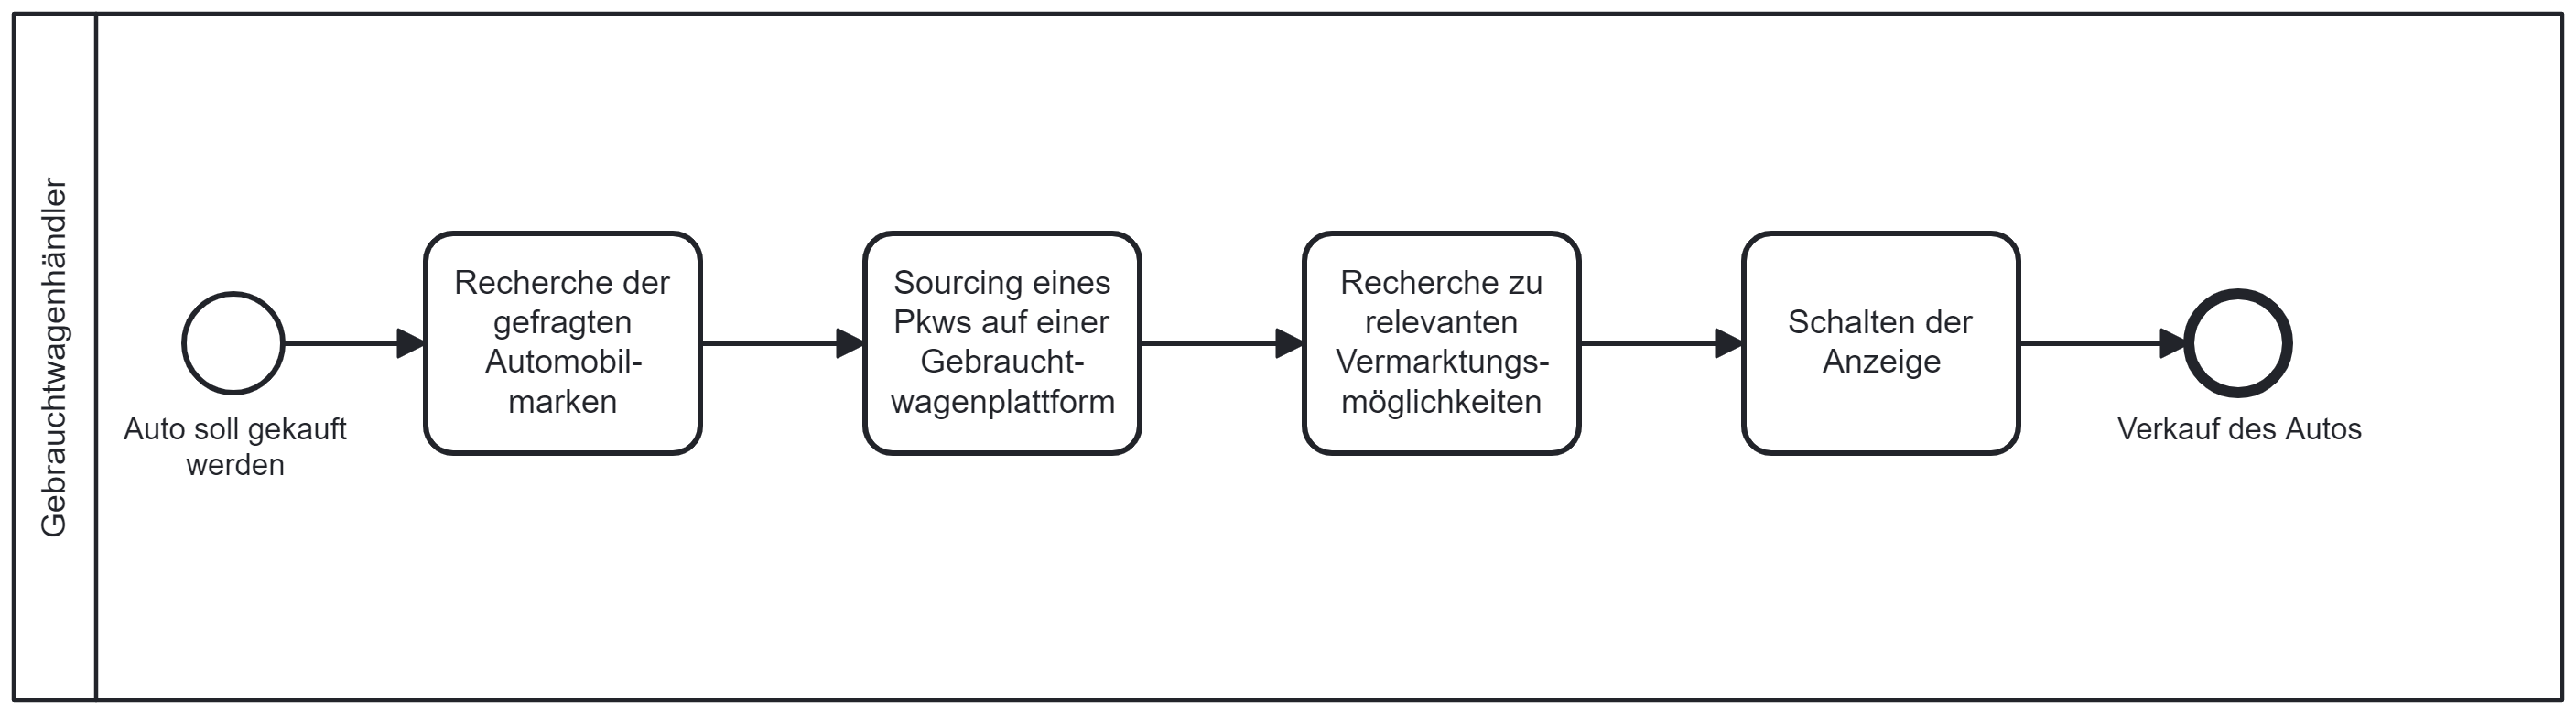
\includegraphics[width=\textwidth]{img/verkaufsprozess.png}
    \caption{Modellierung eines Geschäftsprozess eines Gebrauchtwagenhändlers mit Camunda Modeler}
    \label{fig:business-process}
\end{figure}
Anhand dieses Prozesses werden verschiedene Anwendungsfälle entwickelt, mit denen die Nützlichkeit der oben vorgestellten Visualisierungen erläutert werden soll: \\
\begin{itemize}
    \item Recherche einer relevanten Marke
    \item Recherche einer relevanten Anzeige
    \item Schalten einer optimierten Anzeige
\end{itemize}
\subsection{Starplot: Recherche einer relevanten Marke }

Um eine Vorauswahl zu tre
\subsection{Scatterplot: Recherche einer relevanten Anzeige }
\subsection{Parallelplot: Schalten einer optimierten Anzeige}